\subsection{Bienvenida del administrador de 4MAT}

Se muestra la interfaz de bienvenida.
	\begin{figure}[hbtp]
		
		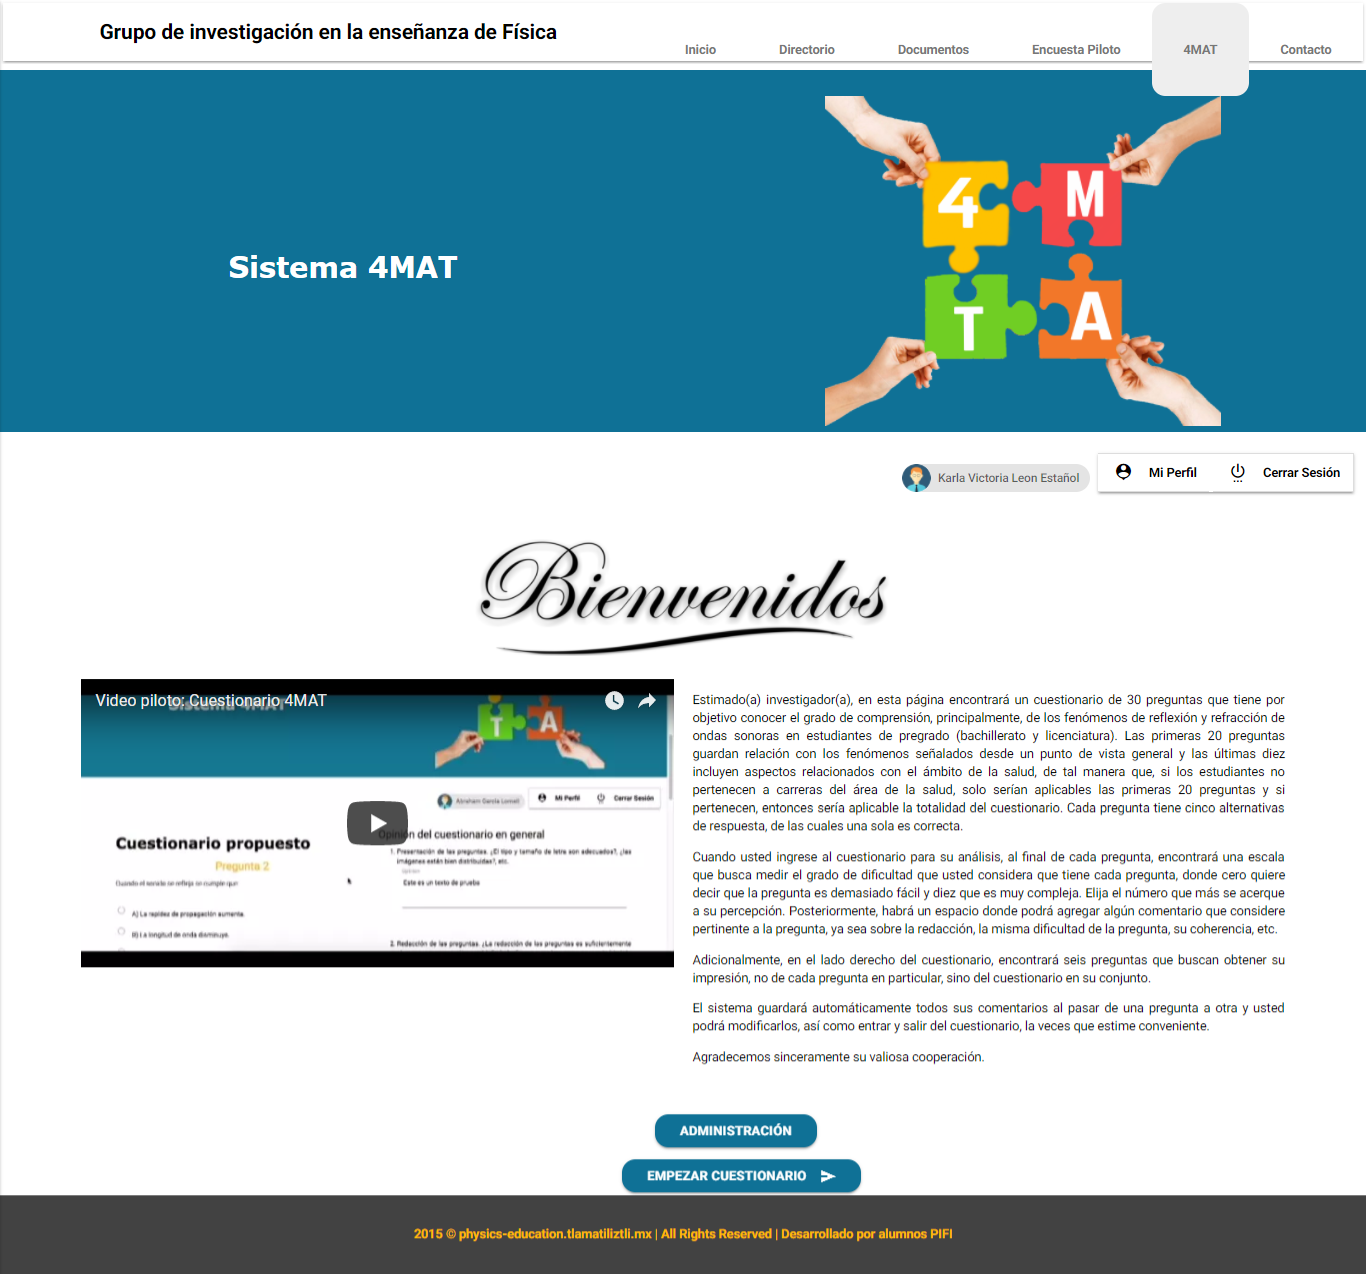
\includegraphics[scale=0.3]{images/Interfaz/IUGS01_binevenida.png}
		\caption{Bienvenida para Administrador}
	\end{figure}
	
La cual contiene los siguientes elementos:
	\begin{itemize}
		\item Menú para las demás secciones de la pagina
			\begin{figure}[hbtp]
		
			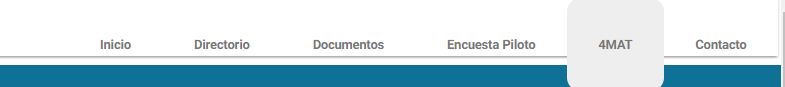
\includegraphics[scale=0.6]{images/Interfaz/IUGS01_menu.png}
			\caption{Menú}
		\end{figure}
		\item Menú de administración de usuario.
			\begin{figure}[hbtp]
		
			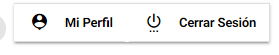
\includegraphics[scale=0.6]{images/Interfaz/IUGS01_menuadmin.png}
			\caption{Menú para datos personales}
		\end{figure}
		
		\item Vídeo explicando como usar la pagina web
		 \begin{figure}[hbtp]
		
			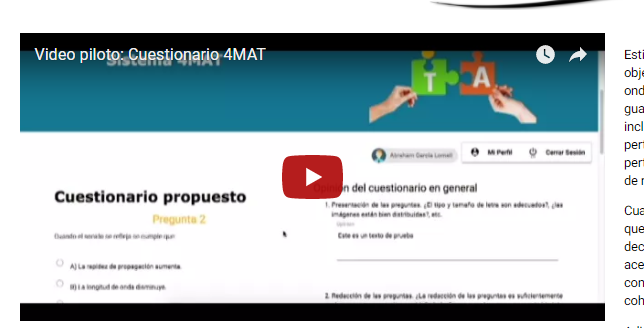
\includegraphics[scale=0.6]{images/Interfaz/IUGS01_video.png}
			\caption{Vídeo explicativo}
		\end{figure}
		\item Botón de administración para consultar estadísticas.
			 \begin{figure}[hbtp]
		
			
\includegraphics[scale=0.6]{images/Interfaz/IUGS01_botonadmin.png}
			\caption{Botón de administración}
		\end{figure}
		\item Botón de iniciar cuestionario. Donde nos presentará el
		cuestionario que se aplicó a los maestros y estudiantes.
		\begin{figure}[hbtp]
		
			
\includegraphics[scale=0.6]{images/Interfaz/IUGS01_botoncuestionario.png}
			\caption{Botón de Empezar Cuestionario}
		\end{figure}
		
	\end{itemize}
	
	